\documentclass{article}

\usepackage{amsmath, amsthm, amssymb, amsfonts}
\usepackage{thmtools}
\usepackage{graphicx}
\usepackage{setspace}
\usepackage{geometry}
\usepackage{float}
\usepackage{hyperref}
\usepackage[utf8]{inputenc}
\usepackage[english]{babel}
\usepackage{framed}
\usepackage[dvipsnames]{xcolor}
\usepackage{tcolorbox}
\usepackage{listings}
\usepackage{xcolor}

\newcommand{\HRule}[1]{\rule{\linewidth}{#1}}
\newcommand{\dsanote}[1]{\textbf{[dsa: #1]}}

% ------------------------------------------------------------------------------

\begin{document}

% ------------------------------------------------------------------------------
% Cover Page and ToC
% ------------------------------------------------------------------------------

\title{ \normalsize \textsc{}
		\\ [2.0cm]
		\HRule{1.5pt} \\
		\LARGE \textbf{Parallel and Distributed Computing
		\HRule{2.0pt} \\ [0.6cm] \LARGE{Project Report - OpenMP Delivery} \vspace*{10\baselineskip}}
		}
\date{}
\author{\textbf{Authors} \\ 
		Carolina Coelho - 99189\\
		Diogo Melita - 99202\\
		Diogo Antunes - 99210}

\maketitle
\newpage

% ------------------------------------------------------------------------------

\section{Introduction}

The goal for this stage is to parallelize the first version of the
\texttt{life3d} program in the shared-memory model using OpenMP.

\section{Serial Version}

The serial version is the basis for the subsequent implementation, therefore
an overview of algorithm is of use for the discussion that follows. The first
step of solution is to compute the statistics for the first generation of the
grid. After this, for each generation the grid is updated by looking at each cell
and following the game's rules. As this is done, the statistics are recomputed, 
and, at the end of the grid update, the maximum values are also changed according
to the new aggregate numbers.

During the development of the parallel version, some optimization opportunities in the
initial program were discovered, and for this reason the sequential version used for
benchmarking is slightly modified. The relevant changes are the following:

\begin{itemize}
	\itemsep -0.2em
	\item addition of two helper functions (\texttt{prepare} and \texttt{finish})
		to avoid including initialization and printing of the answer in the reported time

	\item access to neighbouring cells (in \texttt{next\_inhabitant}) no longer uses a
		loop, but rather leverages explicit reads to improve data locality and avoid redundant
		computation

	\item the histogram computation after each generation was done in a
		\texttt{for} loop, which was unrolled manually
\end{itemize}

\section{Approach Used}

To decide on which part of the code should be paralelized, Linux's \texttt{perf}
tool was used as follows:

\begin{lstlisting}[language=bash,caption={Example usage of \texttt{perf} to identify
serial performance bottleneck}]

perf record -g ./life3d 3 1024 .4 100
perf report -g

\end{lstlisting}

\texttt{perf}'s report (which can be found in greater detail in Appendix A) shows
that for large problems, most time (more than $95\%$ of the CPU cycles for a
representative run in RNL's lab3p7 machine) is spent in the \texttt{next\_inhabitant}
function (which is part of the grid update step in the algorithm). These results
showed that the focus of the parallelization efforts should be the loop that
computes the new grid state. To achieve this in the
shared-memory model, the loop iterations were split among a team of
threads and each thread was assigned a section of the space for which it should compute the
new inhabitants. Additionally, each thread keeps a private histogram for the count for each
specie in its section of the grid. This private histogram must be aggregated
at the end and used to update the global maximum count values. Obviously, this
work cannot be parallelized in any useful way, so it's not divided among the threads.
As a summary, the parallelized algorithm will follow the same structure as before
- for each generation, a fully parallelized grid update, at the end of which
the threads synchronize to compute the aggregate (which is done by a single thread).

\section{OpenMP Parallelization}

As expected, the code parallelization described previously was implemented
 using OpenMP directives (in particular \texttt{parallel}, \texttt{for}, \texttt{collapse}, 
\texttt{reduction}, and \texttt{single}).

The \texttt{parallel} directive is used to create a team of threads 
that will execute the code inside the block. To achieve the desired
work sharing amongst the threads, the \texttt{for} directive was added
to both to the initial loop that goes through the space to compute the initial
statistics as well as to the grid updating loop. To automate the creation
of a private array for each thread's count and the sum of all histograms at
the end, the \texttt{for} is paired with a \texttt{reduction} clause. As expected,
the latter specifies \texttt{+} as the aggregation operation and the count
array as the variable to aggregate on.

The use of a plain \texttt{for} might however create a load imbalance as it
only splits iterations for the outer-most loop. As an example, consider $n=1000$
and a team of 3 threads. If work-splitting is done only at the outermost level,
the final split will be $333 \times 1000^2$, $333 \times 1000^2$ and $334 \times 1000^2$
(i.e. the last thread gets an extra million entries). To ensure this doesn't happen,
\texttt{collapse(3)} is used.

As already mentioned, after each grid update there's a quick set of tasks that
need to be performed - swapping the pointers of the old and new grids and updating 
the maximum population of each specie. These are in general very quick operations
and that would raise concurrency issues if done in parallel. For this reason,
\texttt{single} is used to ensure that a single thread performs the required
changes to prepare for the next iteration. It should be noted that this doesn't
represent any extra synchronization that might hinder the performance as threads
had to synchronize anyway at the end of the \texttt{for} loop to compute the
aggregate statistics.

A relevant aspect of implementation is determining the placement of the \texttt{for} and 
\texttt{parallel} directives. Two solutions were considered:

\begin{itemize}
	\itemsep -0.2em
	\item only two \texttt{parallel for} directives (one at each three level
		loop)

	\item a single \texttt{parallel} section with two inner \texttt{for}
		directive and a \texttt{single} directive

\end{itemize}

Since the thread team is created at the start of the parallel section, the intuition
favors the second option as it avoids spawning threads in each iteration.
Despite this, the experiments performed on both versions
(Table~\ref{omp-directive-choice}) show that a very high generation count and a
very low value for $n$ is required to find relevant performance differences. 
For this reason, the second option was chosen.

\begin{table}[h!]
	\centering
	\begin{tabular}{| c c c c c c||} 
	 \hline
	 gen\_count & $N$ & density & seed & Option 1 execution time & Option 2 execution time \\ [0.5ex] 
	 \hline\hline
	 100000000 & 4 & 0.4 & 0 & 216.9s & 209.8s \\ 
	 10000000 & 4 & 0.4 & 0 & 21.8s & 20.9s \\ 
	 1000000 & 4 & 0.4 & 0 & 2.2s & 2.1s\\
	 100000 & 16 & 0.4 & 0 & 3s & 3s\\ [1ex] 
	 \hline
	\end{tabular}
	\caption{Execution time for both choices of directives}
	\label{omp-directive-choice}
\end{table}

\section{Results}

To benchmark the parallelized code, the input values presented in Table~\ref{input-values}
were used. The programs were executed in the labs machines, by setting
\texttt{OMP\_NUM\_THREADS} to 1, 2, 4 and 6 in order to correctly test the
speedup of our program for different core counts.

\begin{table}[h!]
	\centering
	\begin{tabular}{||c c c c c||} 
	 \hline
	 Input & gen\_count & $N$ & density & seed  \\ [0.5ex] 
	 \hline\hline
	 1 & 1000 & 64 & 0.4 & 0 \\ 
	 2 & 200 & 128 & 0.5 & 1000 \\
	 3 & 10 & 512 & 0.4 & 0 \\ 
	 4 & 3 & 1024 & 0.4 & 100 \\ [1ex] 
	 \hline
	\end{tabular}
	\caption{Inputs used}
	\label{input-values}
\end{table}

The number of threads, the size of the grid, and the number of generations
was varied and for each configuration, 5 runs were executed on the \texttt{lab3p8}
machine. Table~\ref{execution-times} shows the mean value for the execution
time for each configuration and the mean speedup across the tested inputs for
each version. To better understand, the implementation's scalability, a plot
depicting difference between best possible speedup and empirically observed
speedup is also plotted in Image~\ref{speedup}.

\begin{table}[h!]
	\centering
	\begin{tabular}{||c c c c c c c||} 
	 \hline
	 Version & Number of Threads & Input 1 & Input 2 & Input 3 & Input 4 & Speedup\\ [0.5ex] 
	 \hline\hline
	 serial & $N/A$ & 9.5 & 15.0 & 48.7 & 115.5 & $N/A$ \\ 
	 omp & 1 & 9.4 & 15.0 & 48.3 & 115.2 & 1.0 \\ 
	 omp & 2 & 4.8 & 7.6 & 24.6 & 58.8 & 1.98 \\
	 omp & 4 & 2.5 & 3.9 & 12.6 & 30.1 & 3.84 \\
	 omp & 6 & 1.7 & 2.7 & 8.6 & 20.6 & 5.61 \\ [1ex] 
	 \hline
	\end{tabular}
	\caption{Times of execution, in seconds, of the serial and parallelized versions of the code.}
	\label{execution-times}
\end{table}

\begin{figure}[htbp]
    \centering
    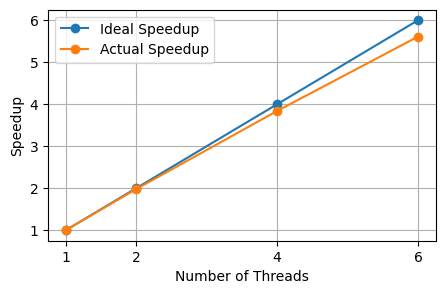
\includegraphics[width=0.5\textwidth]{img/speedup-threads.png}
    \caption{Speedup achieved by the parallelized version when running on different number of threads.}
    \label{speedup}
\end{figure}

As can be seen, the actual speedup is very close to the number of threads
using the program, but gets further from the best possible value as the number
of threads grow. As the code is mostly, but not fully parallelized, this 
observation is according to Amdahl's law and thus the expected behaviour.

To further understand what percentage of the initial program was being parallelized,
the observed behaviour was compared against the one predicted by Amdahl's law
for different portions of the parallelized program. The formula used for this 
purpose is the following ($p$ is the portion of the code that is parallelized and $t$ is 
the number of threads): 

\begin{equation}
	S = \frac{1}{(1-p) + \frac{p}{t}}
\end{equation}

\begin{table}[h!]
	\centering
	\begin{tabular}{||c c c c||} 
	 \hline
	 Parallelized portion & 2 threads & 4 threads & 6 threads \\ [0.5ex] 
	 \hline\hline
	 0.90 & 1.81 & 3.08 & 4.00 \\ 
	 0.95 & 1.90 & 3.48 & 4.80 \\ 
	 0.98 & 1.96 & 3.77 & 5.45 \\ 
	 0.985 & 1.97 & 3.83 & 5.58 \\ 
	 0.99 & 1.98 & 3.88 & 5.71 \\ [1ex] 
	 \hline
	\end{tabular}
	\caption{Times of execution, in seconds, of the serial and parallelized versions of the code.}
	\label{amdahl}
\end{table}

The predictions in Table~\ref{amdahl} suggest that the parallelized portion is
around 98\%, which is very good. This is slightly higher than what would be
expected if the initial \texttt{perf} report was considered, since it suggested
around 95\% of code is in the parallelized section. This slight difference
can be attributed both to some inacurracy on \texttt{perf}'s part and to the
fact that Amdahl's law is a simplification and misses some factors such as the
overhead for parallelization.

\section{Appendix A}

\begin{lstlisting}[caption={\texttt{perf} report on run with $n=1024$ and $3$
generations}]
Samples: 511K of event 'cycles', Event count (approx.): 570685601271
  Children      Self  Command  Shared Object         Symbol
+   89,23%    88,66%  life3d   life3d                [.] next_inhabitant
+    4,46%     4,20%  life3d   life3d                [.] simulation
+    4,27%     3,42%  life3d   life3d                [.] r4_uni
+    3,44%     3,31%  life3d   life3d                [.] gen_initial_grid
     0,26%     0,01%  life3d   [kernel.kallsyms]     [k] asm_exc_page_fault
     0,20%     0,00%  life3d   [kernel.kallsyms]     [k] exc_page_fault
     0,20%     0,00%  life3d   [kernel.kallsyms]     [k] do_user_addr_fault
\end{lstlisting}

\newpage

% ------------------------------------------------------------------------------
% Reference and Cited Works
% ------------------------------------------------------------------------------

\bibliographystyle{IEEEtran}
% \bibliography{References.bib}

% ------------------------------------------------------------------------------

\end{document}
